\documentclass[12pt]{amsart}
% Default margins are too wide all the way around. I reset them here
\setlength{\hoffset}{-.75in}
\setlength{\textwidth}{6.5in}
\setlength{\voffset}{-.5in}
\setlength{\textheight}{9.0in}
\usepackage{amsmath}
\usepackage{amssymb}
\usepackage{amsthm}
\usepackage{pgfplots}
\pgfplotsset{compat=1.18}
\tikzset{orbit/.style={blue!70!black,thick},separatrix/.style={orange!85!black,very thick},field/.style={gray!65,-{Stealth[length=2pt,width=2pt]},line width=.3pt},equilibria/.style={black,very thick}}
\usepackage{enumerate}
\usepackage{tikz}
\usetikzlibrary{shadows,arrows,arrows.meta,shapes,positioning,calc}% Required for the Circle and Triangle arrow tips
\usepackage{setspace}
\usepackage{siunitx}
\usepackage{enumitem}
\usepackage{tcolorbox}
\usepackage{array}
\usepackage{microtype}
\usepackage{hyperref}
\usepackage{upgreek}

\theoremstyle{plain}
\newtheorem{conjecture}{Conjecture}

\theoremstyle{definition}
\newtheorem{definition}{Definition}

\theoremstyle{definition}
\newtheorem{question}{Question}

\theoremstyle{plain}
\newtheorem{theorem}{Theorem}

\newenvironment{solution}
{\begin{proof}[Solution]}
{\end{proof}}

\newcommand{\sectionrule}{%
    \vspace{0.3em}
    \hrule
    \vspace{0.8em}
}


\newcommand{\R}{\mathbb{R}}
\newcommand{\dd}{\mathop{}\!\mathrm{d}}
\newcommand{\vct}[1]{\underline{#1}}
\newcommand{\sys}[2]{\begin{aligned}#1\\#2\end{aligned}}
\newcommand{\rulehead}[1]{\vspace{2pt}\hrule\vspace{5pt}{\large\bfseries #1}\par}

\title{Dynamical Systems:\\Class September 22, 2026\\ 8. Introduction to Limit Cycles}
\author{Rob Tompkins}
\date{September 22, 2026}


\begin{document}

    \maketitle
    {\large\bfseries Teams}

    Post screenshots of your work to the course Google Drive today: Link to drive folder. Include words, labels, and other short notes on your whiteboard that might make those solutions useful to you or your classmates. Name your images using the format:
    \begin{itemize}\item \texttt{teamXX-YY.EXT}\end{itemize}
    where XX is your two-digit team number (e.g. 06 if you are team 6), YY is the two digit number of image for today (e.g. 01 for the first image, 02 for the second, and so on.), and EXT is the extension for the image filetype you used.
    \par\medskip
    {\large\bfseries Team Activity}

    \section*{Problems}

    \begin{enumerate}[label=\arabic*.]
        \item
        \begin{enumerate}[label=(\alph*)]
            \item Sketch a phase portrait for a system with a saddle point at the origin.
            \item Choose a closed curve that encloses the saddle point. Find the index on that curve.
            \item Choose a different closed curve and convince yourself the index is the same.
            \item When a closed curve is a trajectory of the system it has an index of $+1$.
            According to index theory, if the fixed point at the origin in part (a) is the sole
            fixed point in the system, can a closed trajectory exist?
            \item Now add a stable spiral at $(1,0)$. No need to connect the two local pictures up.
            \item Calculate the index about a curve that encircles just the stable spiral.
            \item Could a closed trajectory exist in this new system? If so, where?
        \end{enumerate}

        \begin{solution}
            \begin{enumerate}[label=(\alph*)]
                \item A saddle point has two unstable directions alternating with two stable directions. Thus a local phase portrait at the origin has two trajectories approaching the origin along the stable manifold and two trajectories leaving along the unstable manifold.

                \item As one traverses a closed curve once counterclockwise around the saddle, the vector field makes one net clockwise rotation. Hence
                \[
                    I=-1.
                \]

                \item The index is again $-1$. The particular enclosing curve does not matter as long as it does not pass through a fixed point and can be continuously deformed to the first curve without crossing one.

                \item No. Every closed trajectory has index $+1$, while a curve enclosing only the saddle has index $-1$. Therefore a closed trajectory cannot enclose only this fixed point.

                \item Add a stable spiral at $(1,0)$ to the phase portrait. The saddle remains at the origin and the new stable spiral has index $+1$.

                \item A curve enclosing only the stable spiral has index
                \[
                    I=+1.
                \]

                \item Yes. Index theory permits a closed trajectory surrounding the stable spiral alone, since the enclosed index is $+1$. A curve surrounding only the saddle would have index $-1$, and a curve surrounding both fixed points would have total index $-1+1=0$, so neither could be a closed trajectory.
            \end{enumerate}
        \end{solution}

        \item Find the index of the fixed points.

        \begin{center}
            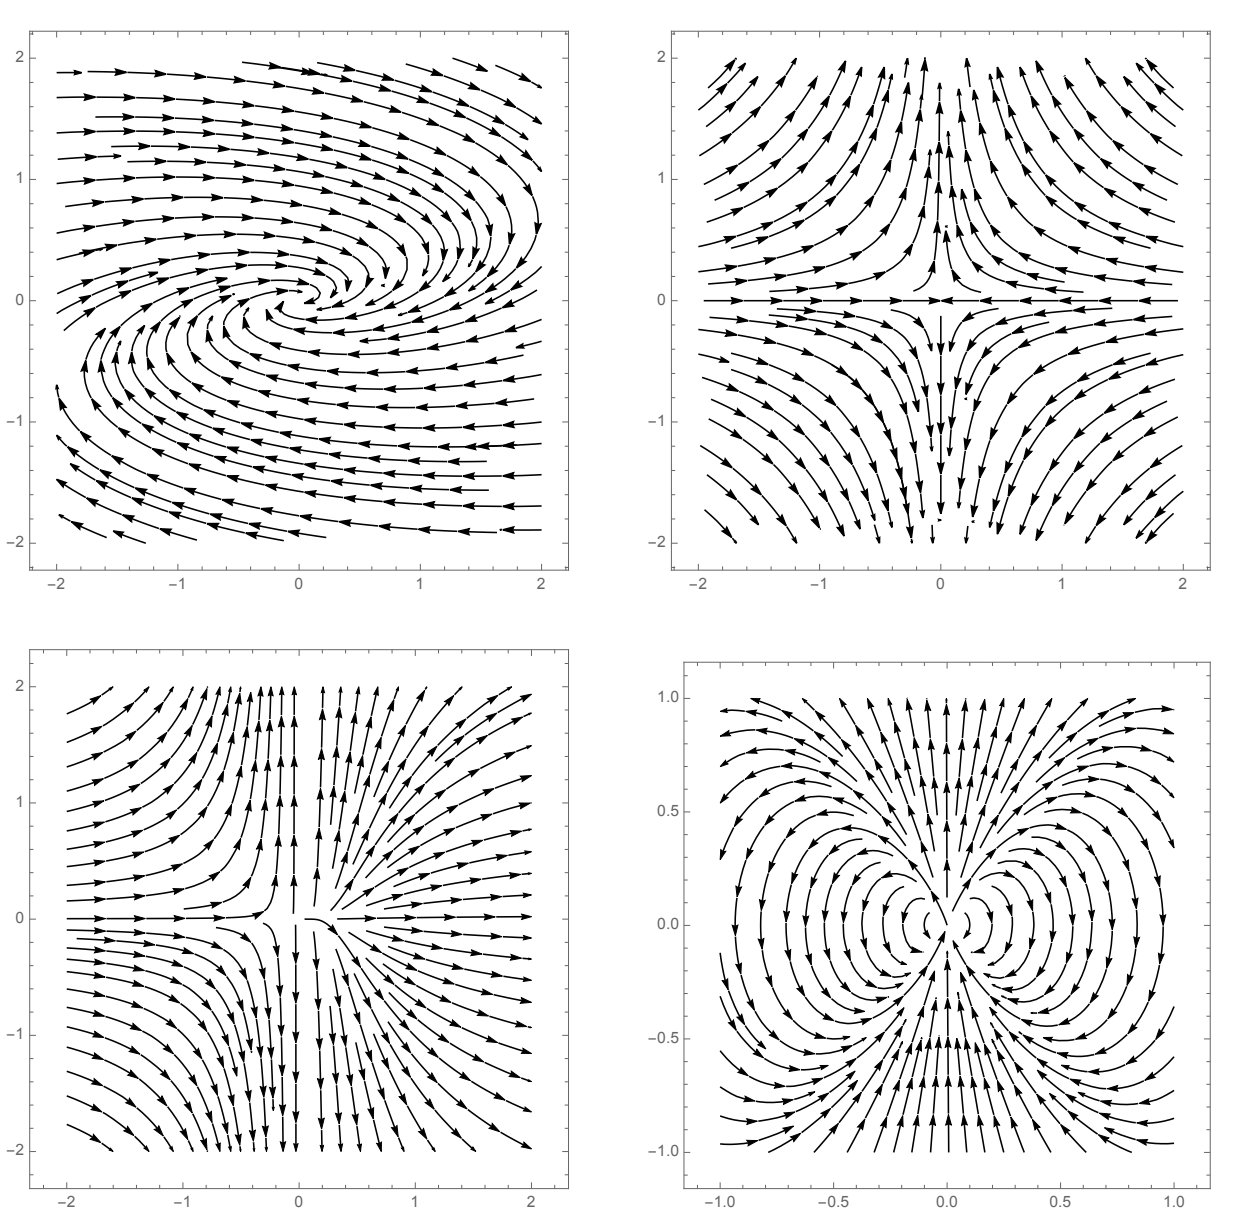
\includegraphics[width=\textwidth]{g08-index-fields.png}
        \end{center}

        \begin{solution}
            The index of a fixed point measures the net number of complete rotations made by
            the vector field as we travel once counterclockwise around a closed curve $C$
            containing the fixed point. Recall that
            \[
                I_f(C)=\frac{\Delta\Theta}{2\pi},
            \]
            where $\Delta\Theta$ is the total change in the angle of the vector field along
            $C$.

            Reading the four phase portraits from upper-left to upper-right, then lower-left
            to lower-right, we obtain the following.

            \begin{enumerate}[label=(\alph*)]
    \item \textbf{Upper-left: $I=+1$.}

    This is a spiral-type fixed point. As we travel once counterclockwise around
    the origin, the direction of the vector field also makes one complete
    counterclockwise rotation. Thus
    \[
        \Delta\Theta=2\pi,
    \]
    and therefore
    \[
        I_f(C)=\frac{2\pi}{2\pi}=+1.
    \]
    The fact that the trajectories spiral rather than form circles does not
    change the index. What matters is that the direction of the vector field
    winds exactly once.

    \item \textbf{Upper-right: $I=-1$.}

    This phase portrait has the characteristic geometry of a saddle point.
    As we travel once counterclockwise around the origin, the vector-field
    direction makes one net rotation in the opposite, clockwise direction.
    Hence
    \[
        \Delta\Theta=-2\pi,
    \]
    so
    \[
        I_f(C)=\frac{-2\pi}{2\pi}=-1.
    \]
    Equivalently, a saddle has four alternating stable and unstable sectors.
    Moving around these sectors produces four net quarter-turns in the negative
    direction, giving one complete clockwise rotation.

    \item \textbf{Lower-left: $I=0$.}

    In this case the direction of the vector field does not make a complete net
    rotation as we travel once around the origin. The vector direction rotates
    one way over part of the circuit and then rotates back over another part, so
    these changes cancel. Therefore
    \[
        \Delta\Theta=0,
    \]
    and
    \[
        I_f(C)=\frac{0}{2\pi}=0.
    \]
    Thus an unusual-looking singularity need not have index $+1$ or $-1$; the
    index depends on the total winding of the vector direction around the
    enclosing curve.

    \item \textbf{Lower-right: $I=+2$.}

    Here, during one counterclockwise trip around the origin, the vector-field
    direction makes two complete counterclockwise rotations. Hence
    \[
        \Delta\Theta=4\pi,
    \]
    and consequently
    \[
        I_f(C)=\frac{4\pi}{2\pi}=+2.
    \]
    Visually, the directional pattern of the arrows repeats twice as we make
    one circuit around the origin, so the vector direction winds twice before
    returning to its initial orientation.
            \end{enumerate}

            Therefore, reading the phase portraits in order from upper-left to upper-right
            and then lower-left to lower-right, their indices are
            \[
                +1,\qquad -1,\qquad 0,\qquad +2.
            \]
            Equivalently, the corresponding total changes in angle are
            \[
                2\pi,\qquad -2\pi,\qquad 0,\qquad 4\pi.
            \]
        \end{solution}

        \item \textbf{(Closed orbits)} Let
        \[
            \dot{x}=y,
            \qquad
            \dot{y}=x-x^3-\delta y+x^2y,
            \qquad \delta\ge0.
        \]
        This system can also be written
        \[
            \ddot{x}=x-x^3-\delta\dot{x}+x^2\dot{x}.
        \]
        This is a variation on the unforced Duffing oscillator (Duffing published work on this
        kind of equation in 1918, and it became a popular model in the 1970s).
        Example taken from Wiggins 2003.

        Use index theory to put limits on where closed trajectories might exist.
        \begin{itemize}
            \item Identify the fixed points.
            \item Use the determinant of the Jacobian matrix to determine the associated index
            for each fixed point.
            \item Sketch all of the possible configurations of closed trajectories in the system,
            based on the index information.
        \end{itemize}

        \begin{solution}
            A fixed point must satisfy
            \[
                y=0,
                \qquad
                x-x^3-\delta y+x^2y=0.
            \]
            Thus, with $y=0$,
            \[
                x-x^3=x(1-x^2)=0,
            \]
            so the fixed points are
            \[
                (0,0),\ (1,0),\ (-1,0).
            \]

            For
            \[
                F(x,y)=
                \begin{pmatrix}
                    y\\
                    x-x^3-\delta y+x^2y
                \end{pmatrix},
            \]
            the Jacobian is
            \[
                J(x,y)=
                \begin{pmatrix}
                    0 & 1\\
                    1-3x^2+2xy & -\delta+x^2
                \end{pmatrix}.
            \]
            Therefore
            \[
                \det J(x,y)=-(1-3x^2+2xy)=-1+3x^2-2xy.
            \]
            At the origin,
            \[
                \det J(0,0)=-1<0,
            \]
            so $(0,0)$ is a saddle and has index $-1$. At the other two fixed points,
            \[
                \det J(\pm1,0)=-1+3=2>0,
            \]
            so each has index $+1$.

            A closed trajectory must have index $+1$. Hence the possible configurations allowed by index theory are:
            \begin{itemize}
                \item a closed trajectory enclosing $(1,0)$ alone;
                \item a closed trajectory enclosing $(-1,0)$ alone;
                \item a closed trajectory enclosing all three fixed points, whose total index is
                \[
                    (+1)+(-1)+(+1)=+1.
                \]
            \end{itemize}
            A closed trajectory cannot enclose the origin alone, nor can it enclose the origin together with exactly one of the other fixed points, because those enclosed indices would be $-1$ and $0$, respectively.
        \end{solution}

        \item \textbf{(Working in polar)}
        Using polar coordinates can be a straightforward way to make a system that is constructed
        to have closed orbits. Consider the system
        \[
            \dot r=r(1-r)(2-r),
            \qquad
            \dot\theta=1.
        \]
        \begin{enumerate}[label=(\alph*)]
            \item We'll think about this system in the $xy$-plane. Note that $\dot\theta=1$, so
            \[
                \theta(t)=t+\theta_0,
            \]
            and we think of it mod $2\pi$. The angle is continuously increasing in the
            counterclockwise direction. This continuous motion in the angle means that, away from
            the origin, there can't be a fixed point.
            \begin{itemize}
                \item What kind of trajectory will you have for this system when $\dot r=0$?
                \item What about if $\dot r=0$ and $r=0$?
            \end{itemize}

            \item To analyze the system, first consider the 1d system
            \[
                \frac{\dd x}{\dd t}=x(1-x)(2-x).
            \]
            What are the fixed points? Sketch what is happening on the $x$-axis.
            Restrict yourself to $x\ge0$.

            \item Now think about the system
            \[
                \dot r=r(1-r)(2-r),
                \qquad
                \dot\theta=1.
            \]
            Show that $r=1$ and $r=2$ are phase curves of the system. Trajectories that start
            on these curves stay on these curves for all time.

            To do this, show that
            \[
                \frac{\dd r}{\dd t}=0
            \]
            when $r=1$ or when $r=2$. Why is this sufficient to show that these curves are
            phase curves?

            \item Sketch in the $\dot r=0$ trajectories. Try to sketch a phase portrait.
        \end{enumerate}

        \begin{solution}
            \begin{enumerate}[label=(\alph*)]
                \item Since $\dot\theta=1$, every point with $r>0$ continually rotates counterclockwise. If $\dot r=0$ for some constant radius $r>0$, then the radius remains fixed while $\theta$ increases, so the trajectory is a circle, hence a closed orbit. If $r=0$, all angular values represent the origin, so the origin is a fixed point.

                \item Consider
                \[
                    \dot x=x(1-x)(2-x),\qquad x\ge0.
                \]
                The fixed points are
                \[
                    x=0,\ 1,\ 2.
                \]
                The signs of $\dot x$ are
                \[
                    \begin{array}{c|ccccccc}
                        x & 0 && 1 && 2 && {}\\ \hline
                        \dot x && + && - && + &
                    \end{array}
                \]
                so the one-dimensional phase line is
                \[
                    0\;\longrightarrow\;1\;\longleftarrow\;2\;\longrightarrow.
                \]
                Thus $r=0$ is unstable, $r=1$ is stable, and $r=2$ is unstable in the radial direction.

                \item For
                \[
                    \dot r=r(1-r)(2-r),
                \]
                substituting $r=1$ gives
                \[
                    \dot r=1(1-1)(2-1)=0,
                \]
                and substituting $r=2$ gives
                \[
                    \dot r=2(1-2)(2-2)=0.
                \]
                Therefore a solution beginning on either circle has constant radius. Since $\dot\theta=1$, it moves around that circle counterclockwise. Hence $r=1$ and $r=2$ are invariant phase curves and closed trajectories.

                \item The radial sign analysis gives
                \[
                    \begin{cases}
                        \dot r>0, & 0<r<1,\\
                        \dot r<0, & 1<r<2,\\
                        \dot r>0, & r>2.
                    \end{cases}
                \]
                Together with $\dot\theta=1$, trajectories rotate counterclockwise. Trajectories with $0<r<1$ spiral outward toward $r=1$, while trajectories with $1<r<2$ spiral inward toward $r=1$. Thus $r=1$ is a stable limit cycle. For $r>2$, trajectories spiral outward away from $r=2$, while just inside $r=2$ they move inward, so $r=2$ is an unstable limit cycle. The origin is an unstable fixed point.
            \end{enumerate}
        \end{solution}
    \end{enumerate}

\end{document}
